\section{Problem Analysis}


%%%%%%%%%%%%%%%%%%%%%%%%%%%%%%%%%%%%%%%%%%%%%%%%%%%%%%%%%%%%%%%%%%%%%%%%%%%%%%%%
\subsection{Available Datasets}

The basis for the analysis is 2 datasets created by Simplesite:
\texttt{EngagementData} \& \texttt{CustomerJourney}. Table
\ref{tab:engdatalayout} and Table \ref{tab:cjdatalayout} names the features of
each dataset and what they represent. Both datasets contain users created
between September 1st 2015 and September 30 2015. \todo{This window can be
expanded as long as the user it at least a month old.} The data is recorded for
all users afterwards as well, but the larger dataset also increases memory
consumption, and makes it unwieldy.

\begin{table}[H]
	\centering
	\begin{tabularx}{\textwidth}{l|X}
		\textbf{Attribute Name} & \textbf{Attribute Data}                                                                                                     \\ \hline
		\textit{islogins1}                       & Bool, true if: one or more logins for the user.                                                            \\
		\textit{islogins2}                       & Bool, true if: two or more logins for the user.                                                            \\
		\textit{islogins3}                       & Bool, true if: three or more logins for the user.                                                          \\
		\textit{islogins4}                       & Bool, true if: four or more logins for the user.                                                           \\
		\textit{isedit30m}                       & Bool, true if: User edited site within 30 minutes of creation.                                             \\
		\textit{isedit24h}                       & Bool, true if: User edited site within 24 hours of creation (excluding the first 30 minutes).              \\
		\textit{isaddpage30m}                    & Bool, true if: User added a new page within 30 minutes of creation.                                        \\
		\textit{isaddpage24h}                    & Bool, true if: User added a new page within 24 hours of creation (excluding the first 30 minutes).         \\
		\textit{isimgupload30m}                  & Bool, true if: User uploaded their own image within 30 minutes of creation.                                \\
		\textit{isimgupload24h}                  & Bool, true if: User uploaded their own image within 24 hours of creation (excluding the first 30 minutes). \\
		\textit{iseditdesign30m}                 & Bool, true if: User edited site within 30 minutes of creation.                                             \\
		\textit{iseditdesign24h}                 & Bool, true if: User edited site within 24 hours of creation (excluding the first 30 minutes).              \\
		\textit{customerid}                      & Integer value with the customers unique ID.                                                                \\
		\textit{marketname}                      & String with the market the user came from (US, TR, DK etc.)                                                \\
		\textit{siteverkey}                      & String with what version of the site the user is created in (US, TR, DK etc.)                              \\
		\textit{ispayer}                         & Bool, true if: The customer have a paid subscription.                                                      \\
		\textit{culturekey}                      & String with language information for the site (en-US, fr-FR etc.)
	\end{tabularx}
	\caption{Features found in the \texttt{EngagementData} dataset.}
	\label{tab:engdatalayout}
\end{table}


\begin{table}[H]
	\centering
	\begin{tabularx}{\textwidth}{l|X}
		\textbf{Attribute Name} & \textbf{Attribute Data}                                                                      \\ \hline
		\textit{customerid}     & Integer value with the customers unique ID.                                                  \\
		\textit{logins14}       & Integer, number of times the customer logged in the first 14 days (week 1-2 after creation). \\
		\textit{logisnw2w4}     & Integer, number of times the customer logged in in week 3-4 after creation.                  \\
		\textit{edits14}        & Integer, number of times the customer edited a page within the first 14 days.                \\
		\textit{iscjtrial}      & Bool, true if: Always true, everyone starts as a trial.                                      \\
		\textit{iscjonboarded}  & Bool, true if: edits14 $\geq 1$.                                                             \\
		\textit{iscjactivated}  & Bool, true if: edits14 $\geq 3$.                                                             \\
		\textit{iscjengaged}    & Bool, true if: edits14 $\geq 6$ and logins14 $\geq 2$.                                       \\
		\textit{iscjinvested}   & Bool, true if: edits14 $\geq 15$ and logins14 $\geq 6$.                                      \\
		\textit{iscjretained}   & Bool, true if: logisnw2w4 $\geq 1$.                                                          \\
		\textit{isimgupload1d}  & Bool, true if: Customer uploaded an image within the first 24 hours of being created.        \\
		\textit{iseditdesign1d} & Bool, true if: Customer edited the design within the first 24 hours of being created.        \\
		\textit{isaddpage1d}    & Bool, true if: Customer added a new page within the first 24 hours of being created.         \\
		\textit{isedit1d}       & Bool, true if: Customer edited a page within the first 24 hours of being created.           
	\end{tabularx}
	\caption{Features found in the \texttt{CustomerJourney} dataset.}
	\label{tab:cjdatalayout}
\end{table}


%%%%%%%%%%%%%%%%%%%%%%%%%%%%%%%%%%%%%%%%%%%%%%%%%%%%%%%%%%%%%%%%%%%%%%%%%%%%%%%%
\subsection{Dataset Pruning}
\label{sec:datasetpruning}

The initial goal is to find customers who are retained (\textit{iscjretained} =
\texttt{True}) and see if there is some pattern, that Simplesite can use to try
to guide other customers down in order to increase the number of retained
customers. With this in mind there is some attributes of the datasets that will
not be helpful, either because they cannot be controlled/changed, or because
they do not make sense. The following is a list of attributes removed from the
\texttt{EngeagementData} dataset during work, along with the reason for the
removal.

\begin{itemize*}
  \item \textit{islogins1} : Removed since it is always true for all customers.

	\item \textit{islogins2} : Removed because the definition of a retained
	      customer requires one or more logins, so this must always be true.

	\item \textit{islogins3} : Same as \textit{islogins2}.

	\item \textit{islogins4} : Same as \textit{islogins2}.

	\item \textit{marketname} : Removed since we are unable to get a customer from
	      a different market, we are insterested in variable we can change for
	      each customer.

	\item \textit{siteverkey} : Same as \textit{marketname}.

	\item \textit{ispayer} : Removed because it is an alternative target variable,
	      it does not say anything about how the user behaves, other than they are
	      indeed a good customer.

	\item \textit{culturekey} : Same as \textit{marketname}.
\end{itemize*}

\noindent The following is a list of attributes removed from the
\texttt{CustomerJourney} dataset during work, along with the reason for the
removal.

\begin{itemize*}
	%\item \textit{logins14} : Removed because initial tests showed high bias. For
	%      a ctree\footnote{Conditional Inference Tree.} of depth 4, the three top
	%      levels was occupied with choices regarding logins14.

	\item \textit{logisnw2w4} : Removed since this attribute is in the definition
	      of our target variable \textit{iscjretained}.

	\item \textit{iscjtrial} : Removed since it is always true.

	\item \textit{iscjonboarded} : Removed since it serves as an alternative
	      target variable, and is set by us, it does not say anything about the
	      user behaviour that is not already present.

	\item \textit{iscjengaged} : Same as \textit{iscjonboarded}.

	\item \textit{iscjinvested} : Same as \textit{iscjonboarded}.
\end{itemize*}

In both datasets the \textit{customerid} attribute is kept in each dataset, even
though it cannot be used as a feature for analysis since each customer have a
unique ID and thus will not yield any patterns, since it can be used to join the
two datasets together.


%%%%%%%%%%%%%%%%%%%%%%%%%%%%%%%%%%%%%%%%%%%%%%%%%%%%%%%%%%%%%%%%%%%%%%%%%%%%%%%%
\subsection{Tree Type}

While researching R, two distinct type of dicision trees came up, an
implementation of regular decision trees that closely follow the method
described in \cite{breiman1}, as well as conditional inference
trees\cite{hothorn2006unbiased}, which I will shorten to \textit{ctree} in this
report.

Both models produce binary trees that can be used to solve classification
problems. Each node in the tree represents a variable and each edge out of the
node contains a ``case'' that tells something about the variable (is it
true/false, $\geq 5$, and so forth). Each leaf of the tree is then a class,
there can be several leafs with the same class, they just represent different
characteristics of the same class.

The main difference between a regular decision tree and a ctree is how it is
created. A regular decision tree will choose to split using information measures
such as seen in Quinlan et. al.\cite[p. 89]{quinlan1986induction}, whereas the
ctree framework will split based on the relationship between the variables and
the covariates. \todo{Write a better explanation without bloating it.(See
\cite{hothorn2006unbiased}.)}

\todo[inline]{Write more here. And create code for the experiment.}

%%%%%%%%%%%%%%%%%%%%%%%%%%%%%%%%%%%%%%%%
\subsubsection{Plotting}
\label{sec:treetypeplot}

Since a big part of the project is for Simplesite to learn about their customers
behaviour on the site, as much as letting a computer learn it, the readability
of the created models became a criteria as well. In order to guage how easy it
was to get information about the models created by the trees I plotted models
created on the same data, using different functions. Figure
\ref{fig:plotcompare} shows the result for the different models and functions.

\begin{figure}
	\centering
  \begin{subfigure}[b]{0.45\textwidth}
    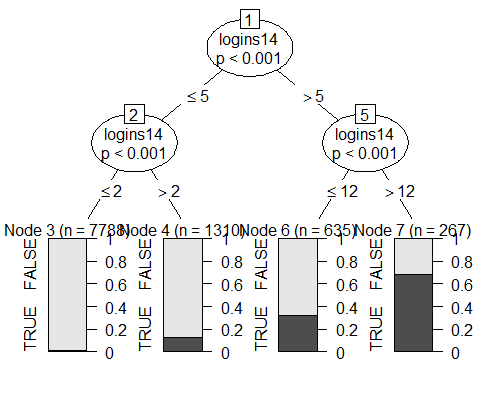
\includegraphics[width=\textwidth]{img/plot_compare_ctree_0}
    \caption{The default plot of a \texttt{ctree} model.}
    \label{fig:plotcompare0}
  \end{subfigure}
  ~ %add desired spacing between images, e. g. ~, \quad, \qquad, \hfill etc.
  \begin{subfigure}[b]{0.45\textwidth}
    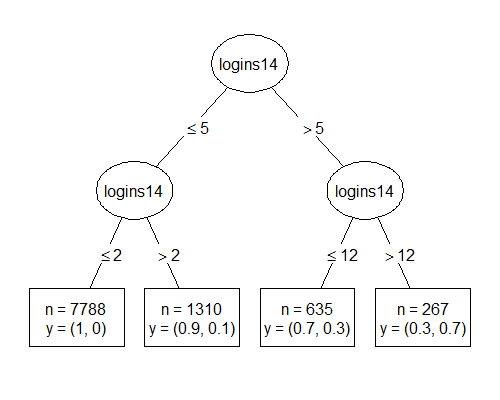
\includegraphics[width=\textwidth]{img/plot_compare_ctree_1}
    \caption{Plot of the same model using a customized plot function.}
    \label{fig:plotcompare1}
  \end{subfigure}


  \begin{subfigure}[b]{0.45\textwidth}
    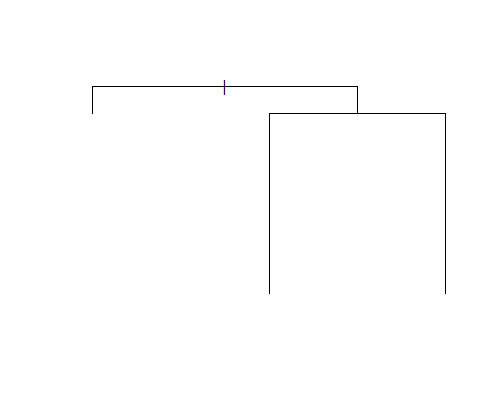
\includegraphics[width=\textwidth]{img/plot_compare_rpart_0}
    \caption{The default plot of a \texttt{rpart} model.}
    \label{fig:plotcompare2}
  \end{subfigure}
  ~
  \begin{subfigure}[b]{0.45\textwidth}
    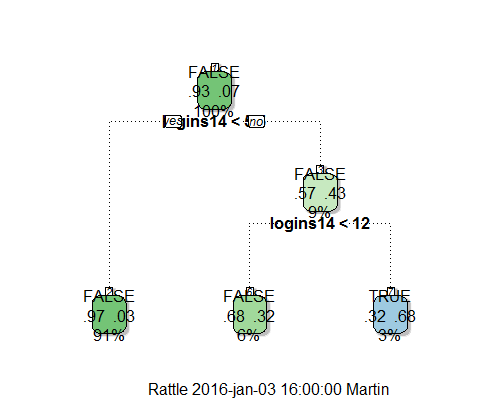
\includegraphics[width=\textwidth]{img/plot_compare_rpart_1}
    \caption{Plot of the same model using \texttt{fancyRpartPlot}}
    \label{fig:plotcompare3}
  \end{subfigure}

  \caption{A side by side view of the different plots produced for the \texttt{
    rpart} and \texttt{ctree} models respectively. Code for creating the figures
    can be found in Appendix \ref{app:code:plotcompare}.}
  \label{fig:plotcompare}
\end{figure}

While which figure is easiest to read can be subjective, I have a few
observations about the figures:
\begin{itemize*}
	\item[\ref{fig:plotcompare0}] Displays the most information of the different
		figures but seems to have issues with being scaled down due to amount of
		information in display.

	\item[\ref{fig:plotcompare1}] Shows most of the information of
	  \ref{fig:plotcompare0} without overflowing.

	\item[\ref{fig:plotcompare2}] Only shows the edges without showing decisions.

	\item[\ref{fig:plotcompare3}] Displays much of the same information as
	  \ref{fig:plotcompare0} and \ref{fig:plotcompare1} but also seems to have
	  problems with scaling.
\end{itemize*}

While all the examples in Figure \ref{fig:plotcompare} are very simple it does
illustrate nicely that some of the plot functions will have trouble later when
the tree grows. Based on the above examples I would use the \texttt{ctree} model
with the plot function from Figure \ref{fig:plotcompare1}.


%%%%%%%%%%%%%%%%%%%%%%%%%%%%%%%%%%%%%%%%
\subsubsection{Model Precision}
\label{sec:treetypeprecision}

In order to make sure that we do not loose any ``precision'' by selecting the
\texttt{ctree} model over the normal decision tree, I performed a number of
tests with each of the models in order to determine if this would indeed be the
case.

For the tests I performed 5-fold cross validation and different maximum tree
depths and recorded the mean precision for each model. The dataset in question
was the combined dataset as described in Section \ref{sec:datasetpruning}
(excluding the customerid column.) The code for this test can be seen in
Appendix \ref{app:code:treecompare}.

\begin{table}[]
	\centering
	\begin{tabular}{l|l|l}
		\textbf{Max Depth} & \textbf{\texttt{rpart} Accuracy} & \textbf{\texttt{ctree} Accuracy} \\ \hline
		\textit{4}         & 0.942799                         & 0.9427990                        \\
		\textit{8}         & 0.942799                         & 0.9431958                        \\
		\textit{12}        & 0.942799                         & 0.9436638                       
	\end{tabular}
	\caption{The mean accuracy for the different 5-fold cross validation runs.}
	\label{tab:treecompare}
\end{table}

The results shown in Table \ref{tab:treecompare} indicates that for our
particular dataset, the accuracy difference for the two models have a very
similar performance in terms of accuracy for our dataset. They both predict
correctly in around $94,3\%$ of the cases with a difference of less that
$0,1\%$ between the best and worst performer.

An interesting observation from the data above is that the \texttt{rpart} model
have the same accuracy for all three runs indicating that the model created does
not change even when it is allowed to grow more complex. After plotting models
from each step, I discovered that it did not grow beyond a depth of 2 and based
itself solely on the \texttt{logins14} variable, similarly to what could be seen
in Figure \ref{fig:plotcompare3}.


%%%%%%%%%%%%%%%%%%%%%%%%%%%%%%%%%%%%%%%%
\subsubsection{Choosing a Model}

Based on the two criteria highlighted in in Sections \ref{sec:treetypeplot} and
\ref{sec:treetypeprecision}, I selected to go with the \texttt{ctree} package,
because it was easier for me to read the information the model was created on
without sacrificing any precision compared to the traditional decision tree
implemented in \texttt{rapart}.


%%%%%%%%%%%%%%%%%%%%%%%%%%%%%%%%%%%%%%%%%%%%%%%%%%%%%%%%%%%%%%%%%%%%%%%%%%%%%%%%
\subsection{Model Analysis}

For this section the two datasets \texttt{EngagementData} \&
\texttt{CustomerJourney} have been joined on the \textit{customerid} attribute,
into one dataset after which the \textit{customerid} attribute was removed. This
is the dataset used for the remainder of this section unless otherwise stated.


%%%%%%%%%%%%%%%%%%%%%%%%%%%%%%%%%%%%%%%%
\subsubsection{Dataset Features}

In section \ref{sec:datasetpruning} I discarded a number of features in the
dataset and reasoned about why they would not be usable for our purpose. This
leaves 14 features as well as the target variable, \texttt{iscjretained}. While
all of these features might be usable


%%%%%%%%%%%%%%%%%%%%%%%%%%%%%%%%%%%%%%%%
\subsubsection{Formula and Tree Depth}

\begin{table}[]
	\centering
	\begin{tabular}{l|l|l}
		\textbf{Formula}                           & \textbf{Max Depth} & \textbf{Mean Accuracy} \\ \hline
		\texttt{iscjretained ~ .}                  & $4$                & 0.9427990              \\
		                                           & $6$                & 0.9429672              \\ % <-- second highest accuracy
		                                           & $8$                & 0.9431958              \\ % <-- highest accuracy
		\texttt{iscjretained ~ edits14}            & $4$                & 0.9350055              \\
		                                           & $6$                & 0.9350227              \\
		                                           & $8$                & 0.9350119              \\
		\texttt{iscjretained ~ logins14}           & $4$                & 0.9427990              \\
		                                           & $6$                & 0.9427990              \\
		                                           & $8$                & 0.9427990              \\
		\texttt{iscjretained ~ edits14 + logins14} & $4$                & 0.9427990              \\
		                                           & $6$                & 0.9428465              \\
		                                           & $8$                & 0.9429414             
	\end{tabular}
	\caption{Mean accuracy of different formulas and tree depths using 5-fold cross
		validation.}
	\label{tab:formulacompare}
\end{table}